% !TEX encoding = UTF-8 Unicode
\documentclass[a4paper]{article}

\usepackage{color}
\usepackage{url}
\usepackage[T2A]{fontenc} % enable Cyrillic fonts
\usepackage[utf8]{inputenc} % make weird characters work
\usepackage{graphicx}

\usepackage[english,serbian]{babel}
%\usepackage[english,serbianc]{babel} %ukljuciti babel sa ovim opcijama, umesto gornjim, ukoliko se koristi cirilica

\usepackage[unicode]{hyperref}
\hypersetup{colorlinks,citecolor=green,filecolor=green,linkcolor=blue,urlcolor=blue}

\usepackage{listings}

%\newtheorem{primer}{Пример}[section] %ćirilični primer
\newtheorem{primer}{Primer}[section]

\definecolor{mygreen}{rgb}{0,0.6,0}
\definecolor{mygray}{rgb}{0.5,0.5,0.5}
\definecolor{mymauve}{rgb}{0.58,0,0.82}

\lstset{ 
  backgroundcolor=\color{white},   % choose the background color; you must add \usepackage{color} or \usepackage{xcolor}; should come as last argument
  basicstyle=\footnotesize,        % the size of the fonts that are used for the code
  breakatwhitespace=false,         % sets if automatic breaks should only happen at whitespace
  breaklines=true,                 % sets automatic line breaking
  captionpos=b,                    % sets the caption-position to bottom
  commentstyle=\color{mygreen},    % comment style
  deletekeywords={...},            % if you want to delete keywords from the given language
  escapeinside={\%*}{*)},          % if you want to add LaTeX within your code
  extendedchars=true,              % lets you use non-ASCII characters; for 8-bits encodings only, does not work with UTF-8
  firstnumber=1000,                % start line enumeration with line 1000
  frame=single,	                   % adds a frame around the code
  keepspaces=true,                 % keeps spaces in text, useful for keeping indentation of code (possibly needs columns=flexible)
  keywordstyle=\color{blue},       % keyword style
  language=Python,                 % the language of the code
  morekeywords={*,...},            % if you want to add more keywords to the set
  numbers=left,                    % where to put the line-numbers; possible values are (none, left, right)
  numbersep=5pt,                   % how far the line-numbers are from the code
  numberstyle=\tiny\color{mygray}, % the style that is used for the line-numbers
  rulecolor=\color{black},         % if not set, the frame-color may be changed on line-breaks within not-black text (e.g. comments (green here))
  showspaces=false,                % show spaces everywhere adding particular underscores; it overrides 'showstringspaces'
  showstringspaces=false,          % underline spaces within strings only
  showtabs=false,                  % show tabs within strings adding particular underscores
  stepnumber=2,                    % the step between two line-numbers. If it's 1, each line will be numbered
  stringstyle=\color{mymauve},     % string literal style
  tabsize=2,	                   % sets default tabsize to 2 spaces
  title=\lstname                   % show the filename of files included with \lstinputlisting; also try caption instead of title
}

\begin{document}

\title{Programski jezik Objective-C\\ \small{Seminarski rad u okviru kursa\\Metodologija stručnog i naučnog rada\\ Matematički fakultet}}

\author{Dalma Beara, Denis Aličić, Mateja Marjanović, Anja Miletić\\ kontakt email prvog, a.denis96@gmail.com, trećeg, anya.miletic@gmail.com}

%\date{9.~april 2015.}

\maketitle

\abstract{
U ovom tekstu je ukratko prikazana osnovna forma seminarskog rada. Obratite pažnju da je pored ove .pdf datoteke, u prilogu i odgovarajuća .tex datoteka, kao i .bib datoteka korišćena za generisanje literature. Na prvoj strani seminarskog rada su naslov, apstrakt i sadržaj, i to sve mora da stane na prvu stranu! Kako bi Vaš seminarski zadovoljio standarde i očekivanja, koristite uputstva i materijale sa predavanja na temu pisanja seminarskih radova. Ovo je samo šablon koji se odnosi na fizički izgled seminarskog rada (šablon koji \emph{morate} da ispoštujete!) kao i par tehničkih pomoćnih uputstava. Pročitajte tekst pažljivo jer on sadrži i važne informacije vezane za zahteve obima i karakteristika seminarskog rada.}

\tableofcontents

\newpage

\section{Uvod}
\label{sec:uvod}

Kada budete predavali seminarski rad, imenujete datoteke tako da sadrže redni broj teme, temu seminarskog rada, kao i prezimena članova grupe. Precizna uputstva na temu imenovnja će biti data na formi za predaju seminarskog rada. Predaja seminarskih radova biće isključivo preko veb forme, a NE slanjem mejla. Link na formu će biti dat u okviru obaveštenja na strani kursa. Vodite računa da prilikom predavanja seminarskog rada predate samo one fajlove koji su neophodni za ponovno generisanje pdf datoteke. To znači da pomoćne fajlove, kao što su .log, .out, .blg, .toc, .aux i slično, \textbf{ne treba predavati}.

\section{Osnovna uputstva}
Vaš seminarski rad mora da sadrži najmanje jednu \textbf{sliku}, najmanje jednu \textbf{tabelu} i najmanje \textbf{sedam referenci} u spisku literature. Najmanje jedna slika treba da bude originalna i da predstavlja neke podatke koje ste Vi osmislili da treba da prezentujete u svom radu. Isto važi i za najmanje jednu tabelu. 	Od referenci, neophodno je imati bar jednu \textbf{knjigu}, bar jedan \textbf{naučni članak} iz odgovarajućeg časopisa i bar jednu adekvatnu \textbf{veb adresu}. 

\textbf{Dužina seminarskog rada treba da bude od 10 do 12 strana.}

\section{Slike i tabele}
\label{slike_i_tabele}

Slike i tabele treba da budu u svom okruženju, sa odgovarajućim naslovima, obeležene labelom da koje omogućava referenciranje. 

Na svaku sliku neophodno je referisati se negde u tekstu. Na primer, na slici \ref{fig:pande} prikazane su pande. 

\begin{primer} I tabele treba da budu u svom okruženju, i na njih je neophodno referisati se u tekstu. Na primer, u tabeli \ref{tab:tabela1} su prikazana različita poravnanja u tabelama.

\begin{table}[h!]
\begin{center}
\caption{Razlčita poravnanja u okviru iste tabele ne treba koristiti jer su nepregledna.}
\begin{tabular}{|c|l|r|} \hline
centralno poravnanje& levo poravnanje& desno poravnanje\\ \hline
a &b&c\\ \hline
d &e&f\\ \hline
\end{tabular}
\label{tab:tabela1}
\end{center}
\end{table}

\end{primer}

\section{Nastanak i istorijski razvoj, mesto u razvojnom stablu, uticaji drugih programskih jezika}
\label{sec:osnovno}

\subsection{Nastanak i istorijski razvoj}
\label{subsec:istorija}
Iako se pojam jezika Objective-C primarno vezuje za proizvode kompanije Epl (engl. Apple) -- MAC OS X, iPhone itd, on je zapravo nastao mnogo pre njih. Njegove temelje postavili su Bred Koks i Tom Lav 1981. godine, težeći da nađu način za povećavanje produktivnosti programera. Te godine pojavio se novi, revolucionarni jezik Smalltalk \cite{smalltalk}, koji je tada unapredio koncept objektno-orijentisanog programiranja. U osnovi tog jezika bilo je posmatranje programa kao skupova objekata koji su mogli da komuniciraju jedni sa drugima dinamički pozivajući metode. To je omogućilo da se stanje programa menja pod uticajem korisnika. Koks je u ovoj ideji video mogućnost da se vrtoglavo ubrza pisanje programa, pošto su se u njemu mogle praviti biblioteke objekata i posle koristiti u drugim programima bez izmene. Međutim, Smalltalk je bio veoma spor i zahtevao je da se svi programi pišu i pokreću u posebnom okruženju. Tada se javila potreba za spajanjem objektno-orijentisanih ideja Smalltalk-a i brzog jezika C. Koks je 1983. objavio naučni rad u kom je predstavio objektno-orijentisani prekompilator (eng.~{\em Object-Oriented Precompiler}). Da bi ovu svoju ideju izbacili na tržište, njih dvojica su osnovali kompaniju Stepstoun (eng.~{\em Stepstone}), izmenili kompilator za OOPC i preimenovali jezik u Objective-C. Iako je glavna ideja ovog projekta bila pisanje i prodavanje pomenutih biblioteka koje su mogle ponovo da se koriste, korisnici su imali dosta zamerki, te je jezik sve više poprimao karakteristike objektno-orijentisanih jezika kakve ih danas znamo, kao što su sakupljač otpada (eng.~{\em garbage collector}) i interpreter, te je kompanija uskoro propala. Stiv Džobs je 1988. kupio licencu, a nekoliko godina kasnije i sva prava za Objective-C za potrebe svoje kompanije NeXT Computer koja se  1996. pripojila Apple-u. Sa tom tranzicijom, sam jezik je pretrpeo razne promene, a najvažnije su uvođenje dveju novih ,,komponenti'': kategorija (eng.~{\em categories}), danas poznatih kao ekstenzije (eng.~{\em extensions}) i protokola (eng.~{\em protocols}). Kategorije su služile da programerima omoguće da sami dodaju funkcije u objekte iz već postojećih biblioteka, a protokoli su omogućavali objektima da komuniciraju jedni s drugima. Oni su danas podržani u jeziku Java i poznati su kao interfejsi (eng.~{\em interfaces}). 

\begin{figure}[h!]
	\begin{center}
	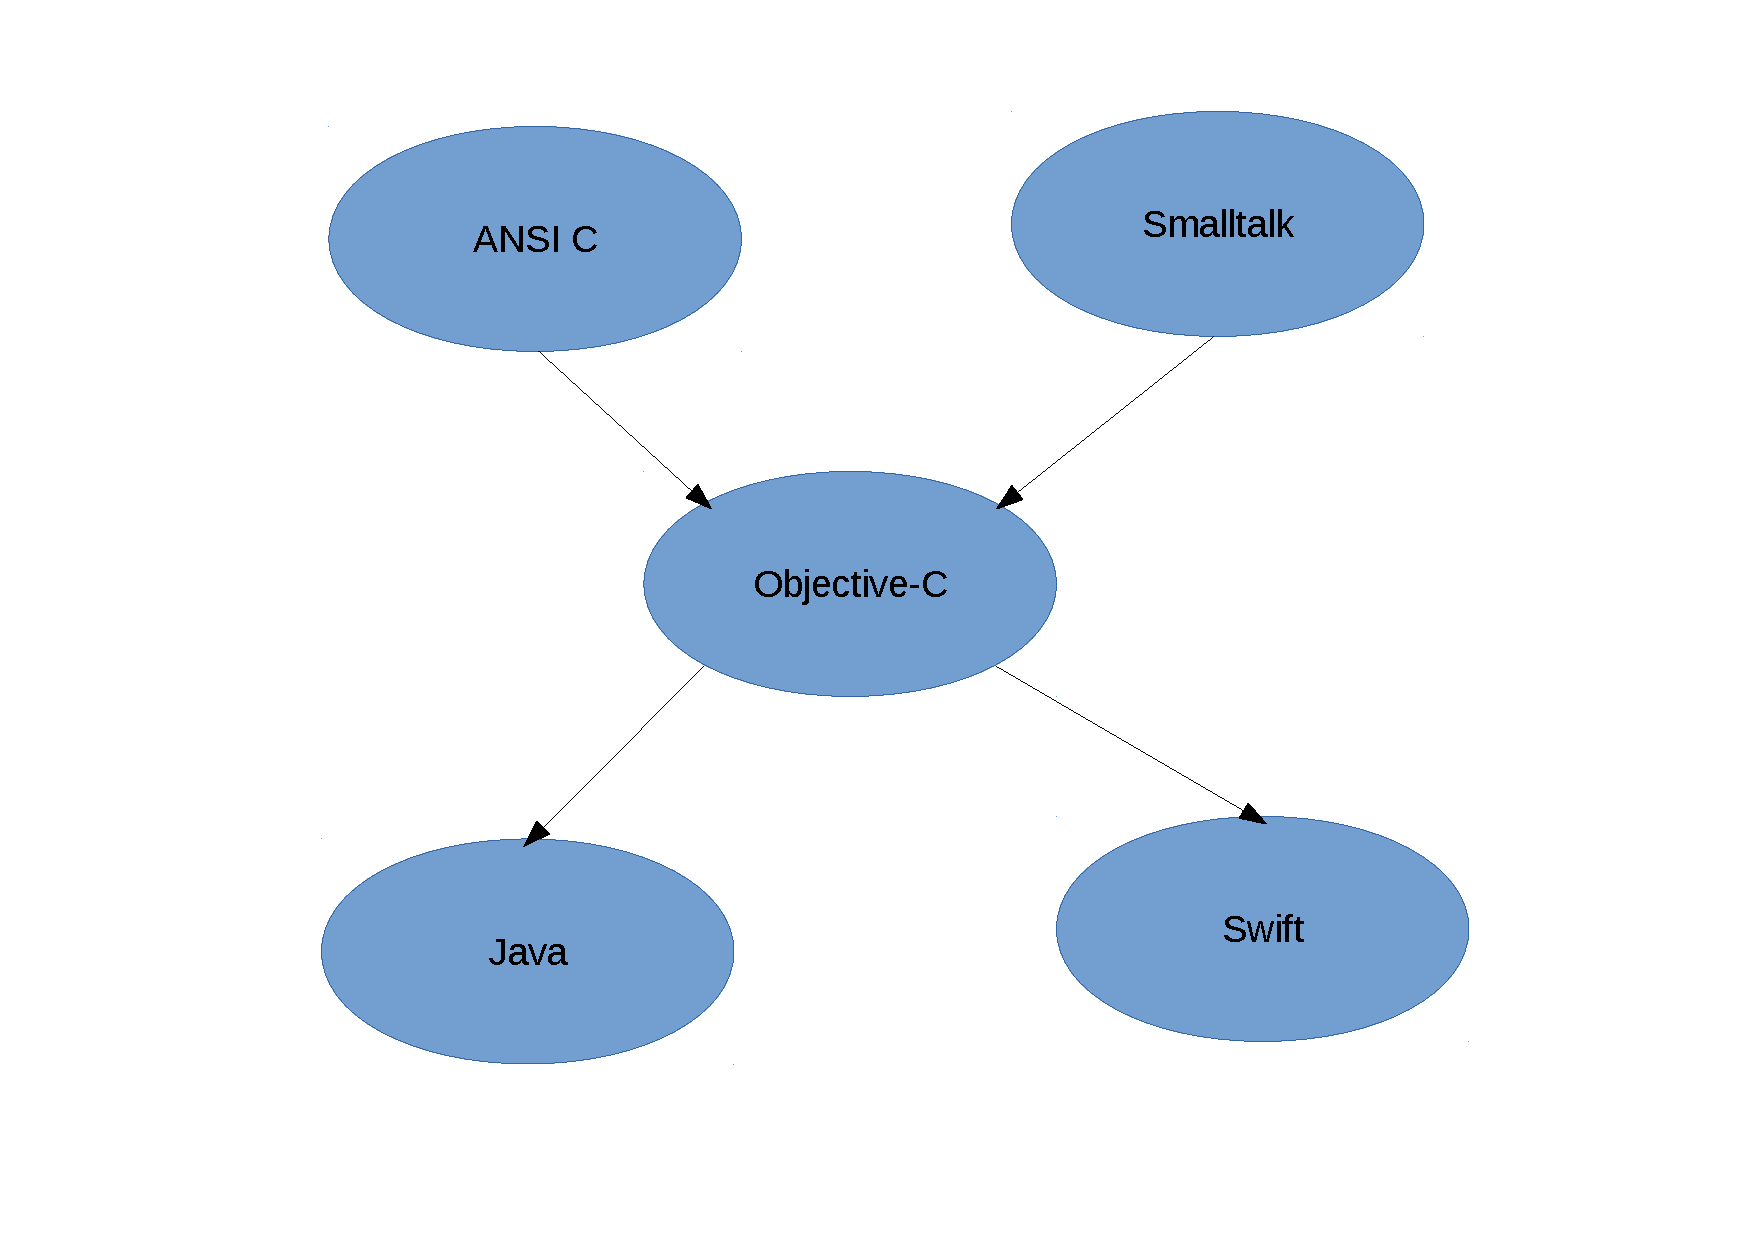
\includegraphics[scale=0.4]{razvojno_stablo.pdf}
	\caption{Razvojno stablo}	
	\label{fig:Razvojno_stablo}
	\end{center}
\end{figure}

\subsection{Uticaj drugih programskih jezika}
\label{subsec:uticaj}
Kao što je već navedeno, Objective-C je nastao kao kombinacija koncepata na kojima počiva Smalltalk utočenih u sintaksu jezika C. Isprva je čak funkcionisao tako što je kod prevođen na C i onda izvršavan. S druge strane, on je uticao na jezik Swift koji je razvio Epl. Swift \cite{swift} se često naziva i ,,Objective-C bez C-a'' kao i na Javu \ref{fig:Razvojno_stablo}. 

\section{Osnovna namena programskog jezika, svrha i mogućnosti}
\label{sec:namena}
Krajem 80-ih godina prošlog veka, popularnost Objective-C jezika je rasla sa razvojem NeXT sistema. Najviše se koristi za razvoj softvera za Apple iOS operativni sistem. Uticaj Objective-C jezika je vidljiv u Java programskom jeziku.
Objective-C definiše mali ali moćan skup ekstenzija ANSI C programskog jezika koje omogućavaju objektno-orijentisano programiranje. Cocoa, Apple-ov API za macOS je napisan uz pomoć Objective-C jezika, takodje veliki deo aplikacija je napisan koristeći taj jezik. 

\section{Osnovne osobine ovog programskog jezika, podržane paradigme i koncepti}
\label{sec:osobine}
Objective-C je nadskup C programskog jezika koji pruža objektno-orijentisane sposobnosti i dinamičko izvršno okruzenje (eng.~{\em runtime}). Objective-C nasledjuje sintaksu, primitivne tipove i naredbe za tok izvršvanja od jezika C, a dodaje sintaksu za definisanje klasa i metoda. Takodje omogućava dinamičko tipiziranje i povezivanje.
\subsection{Osnovni koncepti}
\subsubsection{Klasteri klasa}
Klasteri klasa (eng.~{\em class clusters}) su programski šablon koji se često koristi u pisanju programa na Objective-C jeziku. Klasteri klasa grupišu odredjeni broj privatnih podklasa unutar javne apstraktne nadklase. 
Ovakvo grupisanje pojednostavljuje javno vidljivu arhitekturu objektno-orijentisanih biblioteka i radnih okvira, bez smanjenja njihove funkcionalnosti. Apstraktna nadklasa mora da deklariše metode za kreiranje instanci svojih privatnih podklasa. 
\subsubsection{Introspekcija}
Introspekcija je moćno svojstvo objektno-orijentisanih jezika i okruženja. Ono predstavlja mogućnost objekta da predstavi detalje o sopstvenoj implementaciji u toku izvršavanja programa. Ti detalji mogu biti njegovo mesto u drvetu nasledjivanja, da li implementira odredjeni protokol i da li odgovara na neku poruku. Primer: 
\begin{lstlisting}[frame=single]
while ( id anObject = [objectEnumerator nextObject] ) {
    if ( [self class] == [anObject superclass] ) {
        // do something appropriate...
    }
}
\end{lstlisting}
\subsubsection{Alokacija objekata}
Prilikom alokacije objekata, dodeljuje se zahtevana memorija iz regiona virtualne memorije dostupne programu. Da bi se izračunalo koliko memorije treba alocirati, uzimaju se u obzir instancirane promenjlive tog objekta - uključujući njihove tipove i redosled - kao što je navedeno u klasi objekta.

\subsubsection{MVC}
MVC (eng.~{\em Model-View-Controller}) je programski šablon (eng.~{\em design pattern}) visokog nivoa koji predstavlja globalnu arhitekturu aplikacije i razvrstava objekte prema ulozi koju imaju u toj aplikaciji.
Objektno-orijentisano programiranje ima više koristi od ovog modela; povećava se modularnost korišćenih objekata, njihovi interfejsi su bolje definisani. Sami programi se bolje adaptiraju promeni zahteva.
MVC smatra da postoje tri vrste objekata: model, pogled i kontroler objekti. MVC šablon definiše uloge koje ovi objekti imaju u aplikaciji i način na koji komuniciraju. Pri dizajniranju aplikacije, bitan korak je biranje - ili pravljenje - klasa za objekte koji pripadaju jednoj od ovih uloga. 
\begin{center}
	\makebox[\textwidth]{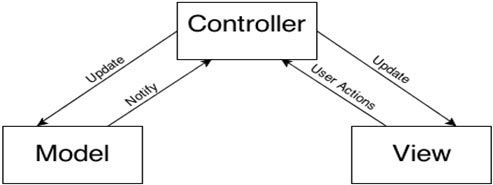
\includegraphics[width=\textwidth]{traditional_mvc1}}
\end{center}

\section{Najpoznatija okruženja (framework) za korišćenje ovog jezika i njihove karakteristike}
\label{sec:okruzenja}

\section{Instalacija i uputstvo za pokretanje na Linux/Windows operativnim sistemima}
\label{sec:instalacija}
\subsection{Instalacija na Linux operativnim sistemima}
\subsubsection{Instalacija neophodnih paketa}
Da bismo mogli da kompajliramo programe napisane u Objective-C, potrebno je prvo da instaliramo
par paketa. Za kompajliranje Objective-C programa koristi se GCC kompajler{\cite{gcc}, uz još par
dodataka.
Prvo što treba da uradimo je da instaliramo GCC podršku za Objective-C.

\begin{lstlisting}[frame=single]
$ sudo apt-get install gobjc
\end{lstlisting}

Zatim treba da instaliramo radno okruženje (eng.~{\em framework}) na kom se moderni Objective-C zasniva i bez kog
ne bi imalo puno smisla raditi (iako je moguće).
To okruženje se zove GNUstep \cite{gnustep} i instalira se komandama:

\begin{lstlisting}[frame=single]
$ sudo apt-get install gnustep
$ sudo apt-get install gnustep-devel
\end{lstlisting}

\subsubsection{Kompajliranje}
Svaki put kada pokrenemo novu sesiju, moramo da pokrenemo skript GNUstep.sh, da bismo mogli da kompajliramo Objective-C programe.
\begin{lstlisting}[frame=single]
$ chmod +x /usr/share/GNUstep/Makefiles/GNUstep.sh
$ /usr/share/GNUstep/Makefiles/GNUstep.sh
\end{lstlisting}

Da ne bismo svaki put morali da izvršavamo taj skript, možemo da uradimo sledeće:

\begin{lstlisting}[frame=single]
$ echo /usr/share/GNUstep/Makefiles/GNUstep.sh >> ~/.bashrc
\end{lstlisting}

I na taj način, svaki put kad se pokrene nova sesija, biće izvršen GNUstep.sh i nećemo morati da brinemo.

Kao što smo već naveli, Objective-C koristi GNU-ov C kompajler, uz dodatnu
podršku.
Sem standardnih argumenata, GCC-u su potrebni i dodatni argumenti (eng.~{\em flags}), kao što su -lobjc, -lgnustep-base, itd.

Dakle ako želimo da prevedemo hello.m program, moramo da izvršimo sledeće:
\begin{lstlisting}[frame=single]
$ gcc hello.m -o hello `gnustep-config --objc-flags` -lgnustep-base -lobjc
\end{lstlisting}

Izvršavanje programa se radi uobičajeno:
\begin{lstlisting}[frame=single]
$ ./hello
\end{lstlisting}

\subsection{Instalacija na Windows operativnim sistemima}

\section{Primer jednostavnog koda i njegovo objašnjenje}
\label{sec:primer}

Zatim, navedimo primer zastarelog (od verzije MAC 10.5), ali zanimljivog koda koji omogućava ,,imitiranje'' (eng.~{\em posing}). 

\begin{lstlisting}[frame=single]
#import <Foundation/Foundation.h>

@interface MyString : NSString

@end

@implementation MyString

- (NSString *)stringByReplacingOccurrencesOfString:(NSString *)target
withString:(NSString *)replacement {
   NSLog(@"The Target string is %@",target);
   NSLog(@"The Replacement string is %@",replacement);
}

@end

int main() {
   NSAutoreleasePool * pool = [[NSAutoreleasePool alloc] init];
   [MyString poseAsClass:[NSString class]];
   NSString *string = @"Test";
   [string stringByReplacingOccurrencesOfString:@"a" withString:@"c"];
   
   [pool drain];
   return 0;
}
\end{lstlisting}

\section{Zaključak}
\label{sec:zakljucak}

Ovde pišem zaključak. 
Ovde pišem zaključak. 
Ovde pišem zaključak. 
Ovde pišem zaključak. 
Ovde pišem zaključak. 
Ovde pišem zaključak. 
Ovde pišem zaključak. 
Ovde pišem zaključak. 
Ovde pišem zaključak. 
Ovde pišem zaključak. 
Ovde pišem zaključak. 
Ovde pišem zaključak. 


\addcontentsline{toc}{section}{Literatura}
\appendix
\bibliography{seminarski} 
\bibliographystyle{plain}



\end{document}
